\part{Numerical errors}
\section{Introduction}
\subsection*{General}
\begin{frame}[label=contents_err]
  \frametitle{Today's outline}
  \mode<beamer>{
    \only<1>{\tableofcontents}
  }
  \only<2>{\tableofcontents[currentsection,currentsubsection]}
\end{frame}

% \begin{frame}
%  \frametitle{Errors in computer programs}
%   In the previous lecture, we have identified three error categories in programming:
%   \begin{description}
%    \item[Syntax errors] You did not obey the language rules. These errors prevent running or compilation of the program.
%    \item[Runtime errors] Something goes wrong during the execution of the program resulting in an error message (problem with input, division by zero, loading of non-existent files, memory problems, etc.)
%    \item[Semantic errors] The program does not do what you expect, but does what have told it to do.
%   \end{description}
%   \pause
%   This is only a subset of all errors that may be encountered:
%   \begin{description}
%    \item[Mathematical model errors] The equations do not describe the physical system
%    \item[Implementation errors] Includes the errors given above
%    \item[Numerical errors] Roundoff, truncation and break errors
%   \end{description}
% \end{frame}

\subsection*{Numerical errors}
\frame{
  \frametitle{Example 1}
  Start your spreadsheet program (Excel, ...) \vskip2em \pause 
  \begin{columns}[T]
    \column{0.5\textwidth}
    Enter: \vskip1em 
    \begin{tabular}{l!{\vrule}c}
        Cell   & Value   \\ \hline
        A1     & \texttt{0.1} \pause \\
        A2     & \texttt{=(A1*10)-0.9} \pause\\
        A3     & \texttt{=(A2*10)-0.9} \pause\\
        A4     & \texttt{=(A3*10)-0.9}
    \end{tabular} \\
    \vskip2em
    (repeat until A30)
    \pause \vskip1em What's happening? \pause

    \column{0.5\textwidth}
    Enter: \vskip1em 
    \begin{tabular}{l!{\vrule}c}
        Cell   & Value  \\ \hline
        A1     & \texttt{2} \pause \\
        A2     & \texttt{=(A1*10)-18}\\
        A3     & \texttt{=(A2*10)-18}\\
        A4     & \texttt{=(A3*10)-18}\\
    \end{tabular}  \\ 
    \vskip2em
    (repeat until A30)
  \end{columns}
}

\begin{frame}[fragile]
  \frametitle{Example 2}
    Start Python \vskip2em \pause 
    Investigate the result of \lstinline$np.sin(1e40 * np.pi)$ \vskip2em \pause
    Create a vector \lstinline$v$ containing the powers of 10, e.g., from $10^0$ up to $10^{40}$, and solve \lstinline$np.sin(v * np.pi)$:
    \begin{lstlisting}[language=Python]
import numpy as np
import matplotlib.pyplot as plt

v = np.logspace(0, 40, 41)
y = np.sin(v * np.pi)
plt.loglog(v, np.abs(y))  # Double log plot, values on y-axis must be positive.
plt.show()
    \end{lstlisting}
\end{frame}

\begin{frame}<1-2>[label=errors]
  \frametitle{Errors in computer simulations}
  In this lecture I will outline different numerical errors that can appear in computer simulations, and how these errors can affect the simulation results.
  \vskip2em
  \pause
  \begin{itemize}[<+->]
  \item Errors in the mathematical model (physics) % Wordt hier niet behandeld, zie FTV/CRE 
  \item Errors in the program (implementation)     % Is behandeld in eerste deel college (bij gebruik debugger)
  \item Errors in the entered parameters           % Wordt hier niet behandeld, zie practicum PT
  \item\alert<7>{ Roundoff- and truncation errors} % Wordt hier behandeld
  \item\alert<7>{ Break errors}                           % Wordt hier behandeld
  \end{itemize}
\end{frame}

\begin{frame}<1-3>[label=verification,fragile]
 \frametitle{Verification and validation}
  \scriptsize\selectfont
  \begin{columns}
    \column{0.6\textwidth}
    \uncover<3->{\begin{block}{Verification}
    Verification is the process of mathematically and computationally assuring that the model computes the equations you intended to implement.
    \end{block}
    }
    \uncover<7->{
    \begin{block}{Validation}
      Validation is the process of determining the degree to which a model is an accurate representation of the real world from the perspective of the intended uses of the model
    \end{block}
    }

  \column{0.4\textwidth}
    \begin{tikzpicture}[block/.style={rectangle,minimum size=3mm,text badly centered,drop shadow,
					thick,rounded corners,draw=maincolor,top color=maincolor!35,bottom color=maincolor!20,
					font=\sffamily\scriptsize},>=stealth,node distance=0.75cm]
	\node[block] (p) at (0,0) {Problem};
	\uncover<2->{\node[below of=p] (p1) {};
	\node[block, below of=p1] (mm) {Mathematical Model};
	\node[below of=mm] (mm1) {};}
	\uncover<4->{\node[block, below of=mm1] (cm) {Computational Model};
	\node[below of=cm] (cm1) {};}
	\uncover<6->{\node[block, below of=cm1] (r) {Results};}
	
	\uncover<3->{\node[block, left of=p1,node distance=2cm] (v1) {Verification};}
	\uncover<5->{\node[block, left of=mm1,node distance=2cm] (v2) {Verification};}
	\uncover<7->{\node[block, left of=cm1,node distance=2cm] (v3) {Validation};}
	
	\uncover<2->{\draw[->] (p) -> (mm);}
	\uncover<4->{\draw[->] (mm) -> (cm);}
	\uncover<6->{\draw[->] (cm) -> (r);}
	
	\uncover<3->{\draw[->] (v1) -> (p1);}
	\uncover<5->{\draw[->] (v2) -> (mm1);}
	\uncover<7->{\draw[->] (v3) -> (cm1);}
    \end{tikzpicture}
  \end{columns}
\end{frame}
% 

\begin{frame}
  \frametitle{Verification of the physical model}
  \scriptsize\selectfont
  \begin{columns}
    \column{0.5\textwidth}
    \begin{center}
      \mode<beamer>{
	\includegraphics<1>[width=0.65\columnwidth]{ptolemy1-1}
	\includegraphics<2>[width=0.65\columnwidth]{ptolemy1-2}
	\includegraphics<3>[width=0.65\columnwidth]{ptolemy1-3}
	\includegraphics<4>[width=0.65\columnwidth]{ptolemy1-4}
	\includegraphics<5>[width=0.65\columnwidth]{ptolemy1-5}
	\includegraphics<6>[width=0.65\columnwidth]{ptolemy1-6}
      }
      \includegraphics<7->[width=0.65\columnwidth]{ptolemy1-7}
    \end{center}
    \column{0.5\textwidth}
    \begin{center}
      \mode<beamer>{
	\includegraphics<7>[width=0.65\columnwidth]{ptolemy2-0}
	\includegraphics<8>[width=0.65\columnwidth]{ptolemy2-1}
	\includegraphics<9>[width=0.65\columnwidth]{ptolemy2-2}
	\includegraphics<10>[width=0.65\columnwidth]{ptolemy2-3}
	\includegraphics<11>[width=0.65\columnwidth]{ptolemy2-4}
	\includegraphics<12>[width=0.65\columnwidth]{ptolemy2-5}
	\includegraphics<13>[width=0.65\columnwidth]{ptolemy2-6}
      }
      \includegraphics<14>[width=0.65\columnwidth]{ptolemy2-7}
    \end{center}
  \end{columns}
    \begin{itemize}
      \setlength{\itemindent}{2cm}
    \item<7-> The perceived orbit of Mars from Earth shows a zig-zag (in contrast to the Sun, Mercury, Venus)
    \item<14> Even though they were not 'right', Earth-centered models (Ptolemy) were still valid
  \end{itemize}
\end{frame}

\begin{frame}
  \frametitle{Be aware of your uncertainties}
  \vfill
  \begin{block}{Aleatory uncertainty}
    Uncertainty that arises due to inherent randomness of the system, features that are too complex to measure and take into account
  \end{block}
  \vskip1em
  \begin{block}{Epistemic uncertainty}
      Uncertainty that arises due to lack of knowledge of the system, but could in principle be known
  \end{block}
  \vfill
\end{frame}

\againframe<2-3>{errors}
\againframe<3-5>{verification}
\againframe<3-4>{errors}
\againframe<5-7>{verification}
\againframe<4->{errors}

\subsection*{Significant digits}
\frame{ 
  \frametitle{Significant digits}
  A numerical result $\tilde{x}$ is an approximation of the real value $x$.
  \begin{itemize}
  \colorize<1>  \item Absolute error
    \[ \delta = \lvert\tilde{x} - x\rvert, x \neq 0 \]
  \colorize<2>  \item Relative error
    \[ \frac{\delta}{\tilde{x}} = \lvert\frac{\tilde{x} - x}{\tilde{x}}\rvert \]
  \colorize<3> \item Error margin 
    \[ \tilde{x} - \delta \leq x \leq \tilde{x} + \delta \] 
    \[ x = \tilde{x} \pm \delta \]
  \end{itemize}
}

\frame{ 
  \frametitle{Significant digits}
  \begin{itemize}
   \colorize<1> \item $\tilde{x}$ has $m$ significant digits if the absolute error in $x$ is smaller or equal to 5 at the $(m+1)$-th position:
   \[ 10^{q-1} \leq \abs{\tilde{x}} \leq 10^q \]
   \[\abs{x-\tilde{x}} = 0.5 \times 10^{q-m}\]
   \colorize<2> \item For example:
   \[ x = \frac{1}{3}, \tilde{x} = 0.333 \Rightarrow \delta = 0.00033333\ldots \]
   3 significant digits
  \end{itemize}
}

\section{Roundoff and truncation errors}
\againframe<2>{contents_err}
\subsection*{roundoff}
\frame{
 \frametitle{Representation of numbers}
 \begin{itemize}[<+->]
  \item Computers represent a number with a finite number of digits: each number is therefore an approximation due to roundoff and truncation errors.
  \item In the decimal system, a digit $c$ at position $n$ has a value of $c \times 10^{n-1}$
 \end{itemize}
 \pause
  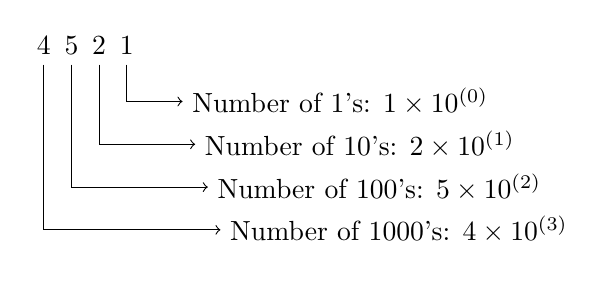
\begin{tikzpicture}[->]
  \node (A) {4};
  \node [right of = A,node distance=10pt] (B) {5};
  \node [right of = B,node distance=10pt] (C) {2};
  \node [right of = C,node distance=10pt] (D) {1};
  
  \node [below right of = D,node distance=1cm,anchor=west] (DD) {Number of 1's: $1 \times 10^{(0)}$};
  \node [below right of = DD,node distance=10pt,anchor=north] (CC) {Number of 10's: $2 \times 10^{(1)}$};
  \node [below right of = CC,node distance=10pt,anchor=north] (BB) {Number of 100's: $5 \times 10^{(2)}$};
  \node [below right of = BB,node distance=10pt,anchor=north] (AA) {Number of 1000's: $4 \times 10^{(3)}$};
  
  \draw (D) |- (DD);
  \draw (C) |- (CC);
  \draw (B) |- (BB);
  \draw (A) |- (AA);
  \end{tikzpicture}
  \pause
  \[ (4521)_{10} = 4 \times 10^3 + 5\times 10^2 + 2 \times 10^1 + 1 \times 10^0 \]
}

% \frame{
%  \frametitle{Representation of numbers}
%  \begin{itemize}[<+->]
%   \item You could use another basis, computers often use the basis 2:
%   \begin{align*}   
%   \hspace*{-1cm}
%  (4521)_{10} = 1& \times 2^{12} + 0 \times 2^{11} + 0 \times 2^{10} + 0 \times 2^9 + 1 \times 2^8 + \ldots \\ 
%   \ldots 1& \times 2^7 + 0 \times 2^6 + 1 \times 2^5 + 0 \times 2^4 + \ldots \\
%   \ldots 1& \times 2^3 + 0 \times 2^2 + 0 \times 2^1 + 1 \times 2^0 \\
%   =& (1000110101001)_2
%   \end{align*}
%   \item In general: 
%   \[ (c_m \ldots c_1 c_0)_q = c_0q^0 + c_1q^1 + \ldots + c_mq^m, c\in\left\{0,1,2,\ldots,q-1\right\} \]
%  \end{itemize}
% }

\frame{
 \frametitle{Representation of numbers}
 \begin{itemize}[<+->]
  \item You could use another basis, computers often use the basis 2:
  \begin{align*}   
  \hspace*{-1cm}
 (4521)_{10} = \onslide<2->{1& \times 2^{12} + \onslide<3->{0 \times 2^{11} + \onslide<4->{0 \times 2^{10} + \onslide<5->{0 \times 2^9 + \onslide<6->{1 \times 2^8 + \ldots \\ 
  \onslide<7->{\ldots 1& \times 2^7 + \onslide<8->{0 \times 2^6 + \onslide<9->{1 \times 2^5 + \onslide<10->{0 \times 2^4 + \ldots \\
  \onslide<11->{\ldots 1& \times 2^3 + \onslide<12->{0 \times 2^2 + \onslide<13->{0 \times 2^1 + \onslide<14->{1 \times 2^0}}}}}}}}}}}}} \\
  =& (\onslide<2->{1\onslide<3->{0\onslide<4->{0\onslide<5->{0\onslide<6->{1\onslide<7->{1\onslide<8->{0\onslide<9->{1\onslide<10->{0\onslide<11->{1\onslide<12->{0\onslide<13->{0\onslide<14->{1)_2}}}}}}}}}}}}}
  \end{align*}
  \onslide<15->{
  \item In general: 
  \[ (c_m \ldots c_1 c_0)_q = c_0q^0 + c_1q^1 + \ldots + c_mq^m, c\in\left\{0,1,2,\ldots,q-1\right\} \]
  }
 \end{itemize}
}

\frame{
 \frametitle{Representation of numbers}
 \begin{itemize}
  \colorize<1> \item Numbers are stored in binary in the memory of a computer, in segments of a specific length (called a \emph{word}).
  \colorize<2> \item We distinguish multiple types of numbers:
  \begin{itemize}
   \colorize<2> \item Integers: $-301, -1, 0, 1, 96, 2293, \ldots$
   \colorize<2> \item Floating points: $-301.01, 0.01, 3.14159265, 14498.2$
  \end{itemize}
  \colorize<3> \item A binary integer representation looks like the following bit sequence:
  \[ z = \sigma \left( c_02^0 + c_12^1 + \ldots + c_{\lambda-1}2^{\lambda-1}\right) \]
  $\sigma$ is the sign of $z$ (+ or -), and $\lambda$ is the length of the word
  \colorize<4> \item Endianness: the order of bits stored by a computer
 \end{itemize}
}

\frame{
 \frametitle{Excercise}
 \begin{itemize}
  \item Convert the following decimal number to base-2: 214 \pause
  \[ 214_{10} = 11010110_2 \] \pause
   \item Excel: 
   \begin{itemize}
     \item Decimal: \texttt{=DEC2BIN(214)}
     \item Octal: \texttt{=DEC2OCT(214)}
     \item Hexadecimal: \texttt{=DEC2HEX(214)}
   \end{itemize}\pause
   \item Python: 
   \begin{itemize}
    \item Decimal: \lstinline$bin(214)$
    \item Octal: \lstinline$oct(214)$
    \item Hexadecimal: \lstinline$hex(214)$
    \end{itemize}
 \end{itemize}
}

\begin{frame}
  \frametitle{Arithmetic operations with binary numbers}
  \centering 
  Addition: \vskip1em
  \begin{columns}
  \column{0.3\textwidth}
    $ 0 + 0 = 0$\\
    $ 0 + 1 = 1$\\
    $ 1 + 0 = 1$\\
    \alert{$ 1 + 1 = 0$ (carry one)}\pause
    \column{0.25\textwidth}
      \begin{tabular}{cccc}
	  & 1 & 4 & 5 \\
	+ &   & 2 & 3 \\
	\hline
	  & 1 & 6 & 8 \\
      \end{tabular}\pause
    \column{0.45\textwidth}
      \begin{tabular}{ccccccccc}
	  & 1 & 0 & 0 & 1 & 0 & 0 & 0 & 1\\
	+ & 0 & 0 & 0 & 1 & 0 & 1 & 1 & 1 \\
	\hline \pause
	  & 1 & 0 & 1 & 0 & 1 & 0 & 0 & 0 \\
      \end{tabular}
  \end{columns}
  \pause
\centering 
\vskip2em  
Subtraction: \\ 
\vskip1em
  \begin{columns}
  \column{0.3\textwidth}
    $ 0 - 0 = 0$\\
    $1 - 0 = 1$\\
    $1 - 1 = 0$\\
    \alert{$0 - 1 = 1$ (borrow one)}\pause
    \column{0.25\textwidth}
      \begin{tabular}{cccc}
	  & 1 & 4 & 5 \\
	- &   & 2 & 3 \\
	\hline
	  & 1 & 2 & 2 \\
      \end{tabular}\pause
    \column{0.45\textwidth}
      \begin{tabular}{ccccccccc}
	  & 1 & 0 & 0 & 1 & 0 & 0 & 0 & 1\\
	- & 0 & 0 & 0 & 1 & 0 & 1 & 1 & 1 \\
	\hline \pause
	  & 0 & 1 & 1 & 1 & 1 & 0 & 1 & 0 \\
      \end{tabular}
  \end{columns}
  \vskip1em
  \begin{itemize}
    \item Multiplication and division are more expensive, and more elaborate
  \end{itemize}
\end{frame}

\frame{
 \frametitle{Exercise}
  Try the following commands in Python:
    \begin{longtable}{l!{\vrule}c}
      Command & Result \\ \hline
      \texttt{np.iinfo(np.int32).min}   & \texttt{-2147483648} \pause \\
      \texttt{np.iinfo(np.int32).max}   & \texttt{2147483647} \pause\\
      \texttt{i = np.int16(np.iinfo(np.int32).max)}   & \texttt{i = 32767} \pause\\
      \texttt{type(i)}   & \texttt{<class 'numpy.int16'>} \pause\\
      \texttt{i = i + 100} & \texttt{i = 32767} \pause\\
      \texttt{np.finfo(np.float64).max} & \texttt{1.7976931348623157e+308} \pause\\
      \texttt{f = 0.1}                  &  \pause\\
      \texttt{type(f)}   & \texttt{<class 'float'>} \pause\\
      \texttt{print("{:.16f}".format(f))} & \texttt{0.1000000000000000} \pause\\
      \texttt{print("{:.20f}".format(f))} & \texttt{0.10000000000000000555}\\
    \end{longtable}
}

{\nologo
\frame{
 \frametitle{Representation of integer numbers}
  \begin{itemize}[<+->]
   \item In Python, integers are typically represented with at least 32 bits (though this can be larger depending on the Python implementation and system architecture). For a typical 64-bit Python installation, the integer type would have 64 bits.
   \item The set of numbers that a 32-bit integer `int32` can represent in numpy is:
   \[
   -2^{31} \leq z \leq 2^{31} - 1 \approx 2\times 10^{9}
   \]
   where \( z \) is a variable representing an \lstinline|np.int32| type value.
   \item If, during a calculation, an integer number in Python exceeds its maximum limit, Python automatically promotes it to a larger type if possible. In the case of numpy, an overflow error will be thrown if a number exceeds the maximum value representable by the `np.int32` type.
   \item How can a computer identify an overflow? Usually through error reporting mechanisms within the language. Python's numpy library, for instance, will throw an OverflowError when an operation results in a number larger than what can be represented by the current data type.
  \end{itemize}
}
}

\begin{frame}[fragile]
 \frametitle{Representation of real (floating point) numbers}
 \begin{itemize}
    \item Formally, a real number is represented by the following bit sequence
    \[ x = \sigma \left( 2^{-1} + c_2 2^{-2} + \ldots + c_m 2^{-m} \right)2^{e-1023} \] \\
    Here, $\sigma$ is  the sign of $x$ and $e$ is an integer value.
  \item A floating point number hence contains sections that contain the sign, the exponent and the mantissa \\
  \vskip1em
    \centering
    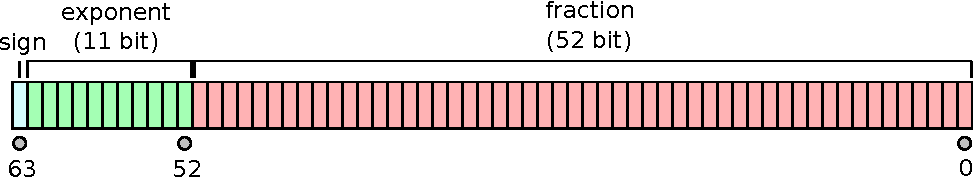
\includegraphics[width=0.9\textwidth]{IEEE_754_Double_Floating_Point_Format}
    \begin{flushright}
    {\tiny
    Image: \href{http://commons.wikimedia.org/wiki/File:IEEE_754_Double_Floating_Point_Format.svg#mediaviewer/File:IEEE_754_Double_Floating_Point_Format.svg}{Wikimedia Commons CC by-SA}} 
    \end{flushright}
 \end{itemize}
\end{frame}

\begin{frame}[fragile]
 \frametitle{Representation of real (floating point) numbers}
 \begin{itemize}
    \item Example: $\lambda = 3$, $m = 2$, $x = \frac{2}{3}$
    \[ x = \pm \left( 2^{-1} + c_2 2^{-2}\right)2^e \]
    \begin{itemize}
      \item $c_0 \in \{0,1\}$
      \item $e = \pm a_0 2^0$
      \item $a_0 \in \{0,1\}$
    \end{itemize}
    \item Truncation: $fl(x) = 2^{-1} = 0.5$
    \item Round off: $fl(x) = 2^{-1} + 2^{-2} = 0.75$
 \end{itemize}
\end{frame}

% \begin{frame}[fragile]
%  \frametitle{Representation of floating point numbers}
%  \begin{columns}
%  \column{0.6\textwidth}
%   \begin{itemize}
%     \item A double is 64 bits (8 bytes)
%     \item Calculate the size of $s$
%     \[ s = \sum_{m=0}^{63} 2^m \onslide<3->{= 1.8447e+19} \]
%   \end{itemize}
%   \pause 
%  \column{0.4\textwidth}
%  \begin{block}{Code example}
%   \begin{lstlisting}
% s = 0;
% for i = 0:63
% s = s + 2^i;
% end
% s
%   \end{lstlisting}
%  \end{block}
%  \pause 
%  \end{columns}
%   \pause
%  \begin{itemize}
%   \item Why is this number smaller than \lstinline$realmax$?
%  \end{itemize}
%  \pause
%  \centering
%  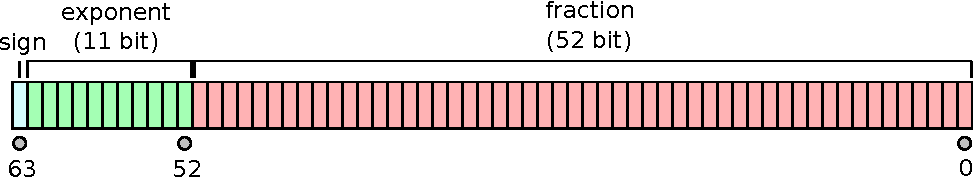
\includegraphics[width=0.9\textwidth]{IEEE_754_Double_Floating_Point_Format}
%    \begin{flushright}
%   {\tiny
%    Image: \href{http://commons.wikimedia.org/wiki/File:IEEE_754_Double_Floating_Point_Format.svg#mediaviewer/File:IEEE_754_Double_Floating_Point_Format.svg}{Wikimedia Commons}} CCA by-SA
%   \end{flushright}
% \end{frame}

\section{Break errors}
\againframe<2>{contents_err}
\subsection*{break}
\begin{frame}
   \frametitle{Trigonometric, Logarithmic, and Exponential computations}
    \begin{itemize}
     \colorize<1> \item Processors can do logic and arithmetic instructions
     \colorize<2> \item Trigonometric, logarithmic and exponential calculations are ``higher-level'' functions:\\
      $\exp$, $\sin$, $\cos$, $\tan$, $\sec$, $\arcsin$, $\arccos$, $\arctan$, $\log$, $\ln$, $\ldots$
      \colorize<3> \item Such functions can be performed using these ``low level'' instructions, for instance using a Taylor series:
      \begin{align*}
        \sin(x) &= \sum_{n=0}^{\infty} \frac{(-1)^n}{(2n+1)!}x^{2n+1} =  x - \frac{x^3}{3!} + \frac{x^5}{5!} - \frac{x^7}{7!} + \ldots \\
         e^x &= \sum_{n=0}^\infty \frac{x^n}{x!} = 1 + x + \frac{x^2}{2!} + \frac{x^3}{3!} + \frac{x^4}{4!} + \ldots
      \end{align*}
    \end{itemize}
\end{frame}

\begin{frame}
   \frametitle{Trigonometric, Logarithmic, and Exponential computations}
    \begin{itemize}
      \colorize<1> \item These operations involve many multiplications and additions, and are therefore \emph{expensive}
      \colorize<2> \item Computations can only take finite time, for infinite series, calculations are interrupted at $N$
    \end{itemize}
%     \hspace*{-2cm} 
    \colorize<2> \begin{flalign*}
      \sin(x) &= \sum_{n=0}^N \frac{(-1)^n}{(2n+1)!}x^{2n+1} =  x - \frac{x^3}{3!} + \frac{x^5}{5!} - \ldots + \frac{(-1)^N}{(2N+1)!}x^{2N+1} & \\
          e^x &= \sum_{n=0}^N \frac{x^n}{x!} = 1 + x + \frac{x^2}{2!} + \frac{x^3}{3!} + \frac{x^4}{4!} + \ldots + \frac{x^N}{N!} &
    \end{flalign*}
    \begin{itemize}
      \colorize<3> \item This results in a \emph{break error}
    \end{itemize}
\end{frame}

\begin{frame}
  \frametitle{Algorithm for sine-computation}
  A computer may use a clever algorithm to limit the number of operations required to perform a higher-level function. A (fictional!) example for the computation of $\sin(x)$:\\
  \begin{columns}
    \column{0.5\textwidth}
    \begin{enumerate}[<+->]
      \item<2-> Use periodicity so that $0 \leq x \leq 2\pi$
      \item<3-> Use symmetry ($0\leq x \leq \frac{\pi}{2}$)
      \item<4-> Use lookup tables for known values
      \item<5-> Perform taylor expansion
    \end{enumerate}

    \column{0.5\textwidth}
    \begin{tikzpicture}[font=\tiny]
      % Grid
      \draw[gridline,step=0.5] (-1,-2) grid (3,2);
      % Axes
      \draw[thick,->] (-1,0) -- (3,0) node[anchor=north west] {$x$};
      \draw[thick,->] (0,-2) -- (0,2) node[anchor=south east] {$y$};
      % Ticks
      \foreach \x in {-1,-0.5,...,2.5}
	\draw (\x cm,1pt) -- (\x cm,-1pt) node[anchor=north] {};
      \foreach \y in {-1,-0.5,...,1.5}
	\draw (1pt,\y cm) -- (-1pt,\y cm) node[anchor=east] {};
      % Ticks (labels)
      \node [anchor=north east] (0,0) {$0$};
      \node [anchor=north ] at (0.5,0) {$\frac{\pi}{2}$};
      \node [anchor=north ] at (1  ,0) {$\pi$};
      \node [anchor=north ] at (1.5,0) {$\frac{3\pi}{2}$};
      \node [anchor=north ] at (2,0) {$2\pi$};
      \node [anchor=east] at (0,-1) {$-1$};
      \node [anchor=east] at (0,1) {$1$};
      % Full graph
      \draw<1> [graph,domain=-1:3] plot (\x, {sin(\x * pi r)});
      % Periodicity
      \draw<2-> [graph,opacity=0.2,domain=-1:3] plot (\x, {sin(\x * pi r)});
      \draw<2> [graph,domain=0:2] plot (\x, {sin(\x * pi r)});
      % Symmetry
      \draw<3-> [graph,domain=0:0.5] plot (\x, {sin(\x * pi r)});
      \node<3> [dot] at (1.8333,-0.5) (c1) {};
      \node<3> [dot] at (1.1667,-0.5) (c2) {};
      \draw<3>[<-] (c1) -- +(0.3,-0.4) node [anchor=west] (c) {$-\sin(x) = c$};
      \draw<3>[<-] (c2) -- (c.west);
      \node<3> [dot] at (0.8333,0.5)  (c3) {};
      \node<3> [dot] at (0.1667,0.5)  (c4) {};
      \draw<3>[<-] (c3) -- +(0.5,0.2) node [anchor=west] (cc) {$\sin(x) = c$};
      \draw<3>[<-] (c4) -- (cc.west);
      % Lookup table
      \node<4> [dot] at (0,0) (p1) {};
      \node<4> [dot] at (0.5,1) (p2) {};
      \node<4> [dot] at (0.25,0.7071) (p3){};
      \draw<4>[<-] (p1) -- +(0.2,-0.7) node [anchor=west] {$\sin(0)=0$};
      \draw<4>[<-] (p2) -- +(0.2,0.4) node [anchor=south west] {$\sin(\frac{\pi}{2})=1$};
      \draw<4>[<-] (p3) -- +(0.5,0.1) node [anchor=west] {$\sin(\frac{\pi}{4})=\frac{1}{2}\sqrt{2}$};
      % Taylor expansion (I had to break up the faculty numbers, they were too large for LaTeX)
      \draw<5-> [graph,opacity=0.4,tuesteel,domain=-0.5*pi:0.5*pi] plot (\x/pi, { ( \x});%
      \node<5> [] at (2,1.7) {$N=0$};
      \draw<6-> [graph,opacity=0.5,tuesteel,domain=-pi:pi] plot (\x/pi, { ( \x - \x*\x*\x/6)});%
      \node<6> [] at (2,1.7) {$N=1$};
      \draw<7-> [graph,opacity=0.6,tuesteel,domain=-pi:pi] plot (\x/pi, { ( \x - \x*\x*\x/6 + \x*\x*\x*\x*\x/120)});%
      \node<7> [] at (2,1.7) {$N=2$};
      \draw<8-> [graph,opacity=0.7,tuesteel,domain=-pi:pi] plot (\x/pi, { ( \x - \x*\x*\x/6 + \x*\x*\x*\x*\x/120 - \x*\x*\x*\x*\x*\x*\x/5040)});%
      \node<8> [] at (2,1.7) {$N=3$};
%  	\draw<5-> [opacity=0.9,smooth,samples=2000,tuesteel,densely dotted,domain=-pi:pi] plot (\x/pi, { ( \x - \x*\x*\x/6 + \x*\x*\x*\x*\x/120 - \x*\x*\x*\x*\x*\x*\x/5040 + \x*\x*\x*\x*\x*\x*\x*\x*\x/40/9072)});% +pow(9,\x)/40/9072 -pow(11,\x)/12474/3200 )});
    \end{tikzpicture}
  \end{columns}
\end{frame}

\section{Loss of digits}
\againframe<2>{contents_err}
\subsection*{loss of digits}
\frame{ 
  \frametitle{Loss of digits}
  \begin{itemize}
    \item During operations such as $+$, $-$, $\times$, $\div$, an error can add up
    \item Consider the summation of $x$ and $y$
     \[ \tilde{x} - \delta \leq x \leq \tilde{x} + \delta \quad \mathrm{and} \quad \tilde{y} - \varepsilon \leq y \leq \tilde{y} + \varepsilon \]
     \[ (\tilde{x} + \tilde{y}) - (\delta + \varepsilon) \leq x + y \leq (\tilde{x} + \tilde{y}) + (\delta + \varepsilon) \]
  \end{itemize}
}

\frame{ 
  \frametitle{Loss of digits: Example 1}
  \[\left.
  \begin{aligned}
    x &= \pi, \tilde{x} = 3.1416\\
    y &= 22/7, \tilde{y} = 3.1429
  \end{aligned} \pause \right\} \Rightarrow 
  \left.
  \begin{aligned}
    \delta &= \tilde{x} - x = 7.35\times10^{-6}\\
    \varepsilon &= \tilde{y} - y = 4.29\times10^{-5}
  \end{aligned} \right\}
\]
\pause
\[ x + y = \tilde{x} + \tilde{y} \pm (\delta + \varepsilon) \approx 6.2845-5.025\times10^{-5} \]
\[ x - y = \tilde{x} - \tilde{y} \pm (\delta + \varepsilon) \approx -0.0013 + 3.55\times10^{-5}\]
  \begin{itemize}
  \item The absolute error is small ($\approx 10^{-5}$), but the relative error is much bigger (0.028).
  \item Adding up the errors results in a loss of significant digits!
  \end{itemize}
}

\frame{ 
  \frametitle{Loss of digits: Example 2}
  \begin{itemize}
    \colorize<1> \item Calculate $e^{-5}$
    \begin{itemize}
      \colorize<1> \item Use the Taylor series
      \colorize<1> \item Calculate the first 26 terms ($N=26$)
    \end{itemize}
    \colorize<2> \item Now repeat the calculation, but use for each calculation only 4 digits. What do you find? \\
    \onslide<2->{Use: \lstinline$round(term, 4)$}
    \colorize<3> \item Without errors you would find: $e^{-5} = 0.006738$
    \colorize<4> \item If you only use 4 digits in the calculations, you'll find 0.00998
  \end{itemize}
}


\frame{ 
  \frametitle{Badly (ill) conditioned problems}
  We consider a system $F(x,y)$ that computes a solution from input data. The input data may have errors:\\ \vskip1em
  \begin{tikzpicture}
    \node [block] (func) {$F(x,y)=0$};
    \node [left of=func,node distance=4cm,anchor=east] (in) {};
    \node [right of=func,node distance=4cm,anchor=west] (out) {(Without errors)};
    \draw [->] (in) -- (func) node[midway,above] {$x$};
    \draw [->] (func) -- (out) node[midway,above] {$y$};
  \end{tikzpicture} \vskip1em \pause
  \begin{tikzpicture}
    \node [block] (func) {$F(x+\delta x,y+\delta y)=0$};
    \node [left of=func,node distance=4cm,anchor=east] (in) {};
    \node [right of=func,node distance=4cm,anchor=west] (out) {(With errors)};
    \draw [->] (in) -- (func) node[midway,above] {$x + \delta x$};
    \draw [->] (func) -- (out) node[midway,above] {$y + \delta y$};
  \end{tikzpicture}\pause
  \begin{columns}
  \column{0.55\textwidth}
  \[ y(x+\delta x) - y(x) \approx y'(x)\delta x \] 
  Propagated error on the basis of Taylor expansion
  \column{0.45\textwidth}
  \[ C = \operatorname*{max}_{\delta x} \left( \left | \frac{\delta y / y}{\delta x / x} \right| \right) \]
  Condition criterion, $C<10$ error development small
  \end{columns}
}

\begin{frame}[fragile]
  \frametitle{Badly (ill) conditioned problems: Example}
  Solve the following linear system in Python using double and single precision:\\
  $ A = 
      \left[\begin{aligned}
       1.2969 & & 0.8648 \\%[0.3em]
       0.2161 & & 0.1441
      \end{aligned}\right], \quad 
     x = \left[\begin{aligned}
       0.8642  \\%[0.3em]
       0.1440 
     \end{aligned}\right]
     \uncover<2->{, \quad 
     y = \left[\begin{aligned}
       2.0 \\%[0.3em]
       -2.0 
     \end{aligned}\right]} $
\begin{columns}[T]
  \column{0.5\textwidth}
  \begin{block}<3->{Double precision}
    \begin{lstlisting}
import numpy as np

# Double precision
A = np.array([[1.2969, 0.8648], [0.2161, 0.1441]], dtype=np.float64)
x = np.array([0.8642, 0.1440], dtype=np.float64)
y = np.linalg.solve(A, x)
print("y =")
print(y)
    \end{lstlisting}
  \end{block}
  \pause 
  \column{0.5\textwidth}
    \begin{block}<4>{Single precision}
      \begin{lstlisting}
import numpy as np

# Single precision
A = np.array([[1.2969, 0.8648], [0.2161, 0.1441]], dtype=np.float32)
x = np.array([0.8642, 0.1440], dtype=np.float32)
y = np.linalg.solve(A, x)
print("y =")
print(y)
    \end{lstlisting}
  \end{block}
\end{columns}
\end{frame}

\frame{ 
\frametitle{Badly (ill) conditioned problems: Example}
\begin{itemize}
  \colorize<1> \item Python does not automatically warn about bad condition number. You need to compute and check it manually using NumPy: \\
  \lstinline$if np.linalg.cond(A) > threshold: raise("Ill conditioned error")$
  \colorize<2> \item The \lstinline$cond$ number is the condition number computed using NumPy.
%   \colorize<2> \item Using Gaussian elimination and fixing the numbers to 11 digits, we find:
%      \[ y = \left[\begin{aligned}
%        0.6662 \\%[0.3em]
%        -0.0002 
%      \end{aligned}\right] \]
    \colorize<3> \item A small error in $A$ (the matrix) results in a big error in the solution. This is called an ill-conditioned problem.
  \end{itemize}
}


\section{(Un)stable methods}
\againframe<2>{contents_err}
\subsection*{Unstable methods}
\frame{
  \frametitle{(Un)stable methods}
  \begin{itemize}
    \item The condition criterion does not tell you anything about the quality of a numerical solution method!
    \item It is very well possible that a certain solution method is more sensitive for one problem than another
    \item If the method propagates the error, we call it an \emph{unstable method}. Let's look at an example.
  \end{itemize}
}

\frame{
  \frametitle{The Golden mean}
  The Golden Mean is a well known ratio and one of the solutions of $\phi^2=\phi+1$, such that $\phi=\frac{1+\sqrt{5}}{2}$, and $\phi-1 = \phi^{-1}$. Many relations to compute $\phi$ have been established (which pose often an interesting source for creating small test programs).
  \begin{itemize}
   \colorize<1> \item Let's evaluate the following recurrent relationship:
    \[ y_{n+1} = y_{n-1} - y_n \]
    \[ y_0 = 1, \quad y_1 = 1-\phi = \phi^{-1} = \frac{2}{1+\sqrt{5}} \]
    \colorize<2> \item Alternatively, a closed form power law relation exists, which again computes $y_n$:
    \[ y_n = x^{-n}, \quad n=0,1,2,\ldots, \quad x = \frac{1 + \sqrt{5}}{2} \]
  \end{itemize}
}
% 
{\nologo
\begin{frame}[fragile]
  \frametitle{The Golden mean}
  \begin{columns}[T]
    \column{0.5\textwidth}
      \begin{block}{Recurrent version}
        \begin{lstlisting}[language=Python]
import numpy as np

def golden_mean_recurrent(Ntot):
    # Initialize the series with the given initial conditions
    y = np.zeros(Ntot)
    y[0] = 1
    y[1] = 2 / (1 + np.sqrt(5))
    
    # Perform the recurrence to fill in the rest of the series
    for n in range(2, Ntot):
        y[n] = y[n-1] - y[n-2]
    return y
        \end{lstlisting}
      \end{block}
    \pause
    \column{0.5\textwidth}
      \begin{block}{Power law version}
        \begin{lstlisting}[language=Python]
import numpy as np

def golden_mean_powerlaw(Ntot):
    # Initialize the constant value
    x = (1 + np.sqrt(5)) / 2
    
    # Generate a range of values from 0 to Ntot and apply the power law
    y = x ** -np.arange(0, Ntot + 1)
    
    return y
        \end{lstlisting}
      \end{block}
  \end{columns}
  \pause
  \begin{itemize}
    \item Compare the outcomes: \lstinline$plot(goldenMeanPowerlaw(40) - goldenMeanRecurrent(40))$ \pause
    \item See what happens if you use single precision (uncomment the second line of both functions).
  \end{itemize}
  \vskip1em
\end{frame}
}
% 
\begin{frame}[fragile]
  \frametitle{The Golden mean}
  \begin{longtable}{c!{\vrule}cc}
    \hline
      $n$   & Recurrent & Power law \\ \hline
      $0$   & $1.0000$ & $1.0000$ \\
      $1$   & $0.6180$ & $0.6180$ \\
      $2$   & $0.3820$ & $0.3820$ \\
      $3$   & $0.2361$ & $0.2361$ \\
      $\ldots$ & $\ldots$ & $\ldots$ \\
      $37$ & $1.714\cdot10^{-08}$ & $1.851\cdot10^{-08}$ \\
      $38$ & $1.366\cdot10^{-08}$ & $1.144\cdot10^{-08}$ \\
      $39$ & $3.485\cdot10^{-08}$ & $7.071\cdot10^{-09}$ \\
      $40$ & $1.017\cdot10^{-08}$ & $4.370\cdot10^{-09}$ \\ \hline
    \end{longtable} 
    \begin{itemize}
      \colorize<2> \item The recurrent approach enlarges errors from earlier calculations!
    \end{itemize}
    \vskip2em
\end{frame}

\frame{
 \frametitle{Example 1: Explanation}
 Recall example 1, where the errors blew up our computation of 0.1, whereas they did not for 2. Why did we see these results? \pause \\ \vskip2em
 \begin{itemize}
 \colorize<2> \item The number 0.1 is not exactly represented in binary
  \begin{itemize}
  \colorize<2> \item A tiny error can accumulate up to catastrophic proportions!
  \end{itemize}
  \colorize<3> \item The number 2 does have an exact binary representation
 \end{itemize}
}

\frame{
    \frametitle{Example 2 (large sine series)}
 
    The \lstinline$np.sin(1e40*np.pi)$ result gives poor results because 1e40 has an error margin on the order of floating-point machine epsilon, which is roughly \(1 \times 10^{-16}\) in Python (double-precision floating-point format). In Python, as in many computing environments, the number of \(2 \cdot \pi\) cycles is still much larger than \(10^{40} \cdot 10^{-16}\). Also, \(\pi\) is not stored with an infinite number of digits, which further contributes to the imprecision.
}

\frame{
 \frametitle{Example 3}
  Start your calculation program of choice (Excel, Python, ...) \vskip1em 
  
  \pause 
  Calculate the result of $y$:
  \[ y = e^{\pi} - \pi \onslide<3->{= 19.999099979\onslide<4->{\neq 20}}\]
  
  \uncover<5>{
  \vskip1em 
  \centering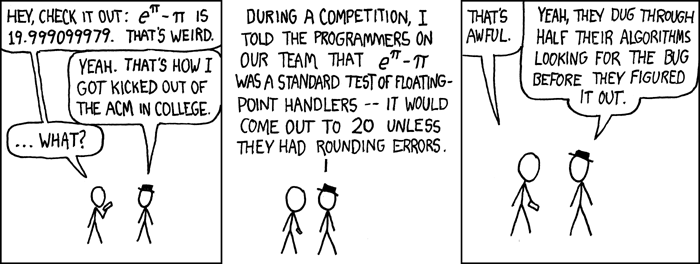
\includegraphics[width=0.8\textwidth]{e_to_the_pi_minus_pi}
  \begin{flushright}
  {\tiny
   Image: \href{http://www.xkcd.com/217/}{xkcd}}
  \end{flushright}
  }
}
 
\section{Symbolic math}
\againframe<2>{contents_err}
\subsection*{Symbolic math}
\frame{ 
  \frametitle{Symbolic math packages}
  \begin{definition}
   The use of computers to manipulate mathematical equations and expressions in symbolic form, as opposed to manipulating the numerical quantities represented by those symbols. 
  \end{definition}
  \vskip1em
  \begin{itemize}
   \item Symbolic integration or differentiation, substitution of one expression into another
   \item Simplification of an expression, change of subject etc.
   \item Packages and toolboxes:
  \end{itemize}
}

\frame{ 
  \frametitle{Symbolic math packages}

   \begin{description}[leftmargin=0.1cm]
    \item[\href{http://www.wolfram.com/mathematica/}{Mathematica}] 
      Well known software package, license available via \href{http://w3.tue.nl/nl/diensten/dienst_ict/services/services_wins/instelling_software/}{TU/e} \vskip0.5em
    \item[\href{http://www.maplesoft.com}{Maple}] 
 Well known, license available via \href{http://w3.tue.nl/nl/diensten/dienst_ict/services/services_wins/instelling_software/}{TU/e}\vskip0.5em
    \item[{\href{http://www.wolframalpha.com/}{Wolfram$|$Alpha}}] 
 Web-based interface by Mathematica developer. Less powerful in mathematical respect, but more accessible and has a broad application range (unit conversion, semantic commands).\vskip0.5em
    \item[\href{http://www.sagemath.org/}{Sage}] 
 Open-source alternative to Maple, Mathematica, Magma, and MATLAB.\vskip0.5em
    \item[\href{http://www.mathworks.nl/help/symbolic/index.html}{Matlab}] 
 Symbolic math toolbox
    \item[\href{https://www.sympy.org/en/index.html}{Python}] 
    SymPy
   \end{description}
}

\lstset{language=Matlab,
    escapeinside={(*@}{@*)}
}

\begin{frame}[fragile]
  \frametitle{Symbolic math: simplify}
  \[ f(x) = (x - 1) (x + 1) (x^2 + 1) + 1 \]
  \pause
  \begin{lstlisting}[language=Python]
from sympy import symbols, simplify

x = symbols('x') # Alt: from sympy.abc import x,y,z
f = (x - 1)*(x + 1)*(x**2 + 1) + 1
f_simplified = simplify(f)
print(f_simplified)
  \end{lstlisting}
  \pause
  \texttt{f\_simplified = x**4}
\end{frame}

\begin{frame}[fragile]
  \frametitle{Symbolic math: integration and differentiation}
  \[ f(x) = \frac{1}{x^3+1} \]
  \pause
  \begin{lstlisting}[language=Python]
from sympy import symbols, simplify, integrate, diff

x = symbols('x')
f = 1/(x**3+1)
my_f_int = integrate(f, x)
my_f_diff = diff(my_f_int, x)
my_f_diff_simplified = simplify(my_f_diff)
print(my_f_diff_simplified)
\end{lstlisting}
  \pause
  \texttt{my\_f\_diff\_simplified = 1/(x**3 + 1)}
\end{frame}

\begin{frame}[fragile]
  \frametitle{Symbolic math: exercises}
  \begin{block}{Exercise 1}
  Simplify the following expression:
  \[ f(x) = \frac{2 \tan x }{(1 + \tan^2 x)} \uncover<2->{ = \sin 2x} \] \vskip-1em
  \pause
  \begin{lstlisting}[language=Python]
from sympy import symbols, trigsimp, tan

x = symbols('x')
expr = 2*tan(x)/(1 + tan(x)**2)
simplified_expr = trigsimp(expr)
  \end{lstlisting}
  \end{block}
\end{frame}

\begin{frame}[fragile]
  \frametitle{Symbolic math: exercises}
  \begin{block}{Exercise 2}
  Calculate the \emph{value} of $p$:
  \[  p = \int_0^{10} \frac{e^x - e^{-x}}{\sinh x}dx \] \vskip-1em
  \pause
  \begin{lstlisting}[language=Python]
from sympy import exp, sinh, integrate, symbols

x = symbols("x")
f = ((exp(x)- exp(-x))/sinh(x)).simplify()
p = integrate(f, (x, 0, 10))
print(p)
  \end{lstlisting}
  \end{block}
  \pause
  \texttt{p = 20}
\end{frame}

{\nologo
\begin{frame}[fragile]
  \frametitle{Symbolic math: root finding }
  A root finding method searches for the values where a function reaches zero. We will cover the numerical methods later, here we show how to use root finding with symbolic math in Python.
   \begin{block}{Symbolic math function}
  \[ f(x) =   \frac{3}{x^2 + 3x} - 2 \]
  \pause
  \begin{lstlisting}[language=Python]
from sympy import solve, symbols

x = symbols("x")
f = 3 / (x**2 + 3*x) - 2
solutions = solve(f, x)
print(solutions)
  \end{lstlisting}
  \end{block}
  \pause
  \texttt{solutions = [-3/2 + sqrt(15)/2, -sqrt(15)/2 - 3/2]}
\end{frame}
}

% \begin{frame}[fragile]
%   \frametitle{Symbolic math toolbox: variable precision arithmetic}
%   Variable precision can be used to specify the number of significant digits.
%       \begin{lstlisting}[language=Python]
% >> from sympy import N

% >> p = N(1/3, 16)
% >> print(p) # 0.3333333333333333
% >> p = N(1/3, 4)
% >> print(p) # 0.3333
% >> a = N(0.1, 30)
% >> print(a) # 0.100000000000000005551115123126
% >> b = N(0.1, 5) 
% >> print(b) # 0.10000
% >> print(a-b) # -0.0000000238418579046051348768742172979
%   \end{lstlisting}
%   \end{frame}

\section{Summary}
\againframe<2>{contents_err}
\subsection*{Summary}
\begin{frame}
  \frametitle{Summary}
  \begin{itemize}
    \colorize<1> \item Numerical errors may arise due to truncation, roundoff and break errors, which may seriously affect the accuracy of your solution
    \colorize<2> \item Errors may propagate and accumulate, leading to smaller accuracy
    \colorize<3> \item Ill-conditioned problems and unstable methods have to be identified so that proper measures can be taken
    \colorize<4> \item Symbolic math computations may be performed to solve certain equations algebraically, bypassing numerical errors, but this is not always possible.
  \end{itemize}

\end{frame}


% References
% http://ocw.mit.edu/courses/electrical-engineering-and-computer-science/6-00sc-introduction-to-computer-science-and-programming-spring-2011/unit-1/lecture-1-introduction-to-6.00/
% http://www.greenteapress.com/thinkpython/html/thinkpython002.html
% https://www.youtube.com/channel/UCLMQ21H2ad95faYG3yGCwYA
%http://stackoverflow.com/questions/4227145/in-matlab-are-variables-really-double-precision-by-default
%http://www.exploringbinary.com/why-0-point-1-does-not-exist-in-floating-point/

